\begin{tikzpicture}[->, >=stealth, node distance=1cm, auto, scale=1, transform shape]
    % Piranha Plants score snippet
    \node [inner sep=0pt] (notes) {
        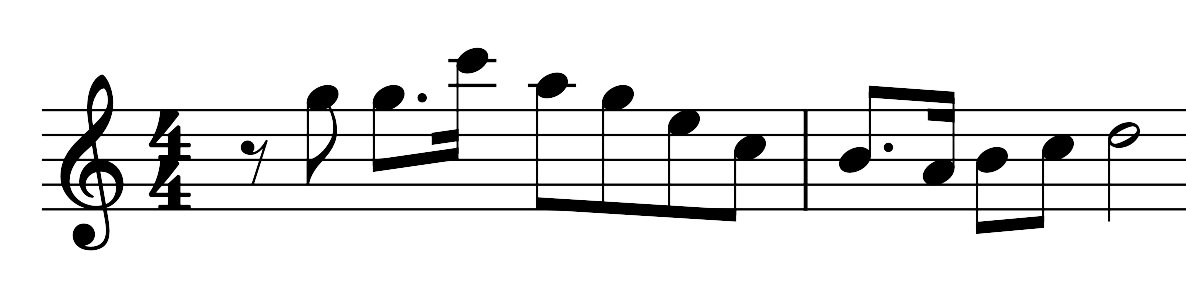
\includegraphics[width=7cm]{figures/piranha_plants_snippet.png}
    };

    \node[draw, red, thick, anchor=north west, minimum width=1.7cm, minimum height=1.3cm] (notes1) at ([xshift=1.25cm, yshift=-0.1cm] notes.north west) {};
    \node[draw, blue, thick, anchor=north west, minimum width=1.6cm, minimum height=1.3cm] (notes2) at ([xshift=3cm, yshift=-0.1cm] notes.north west) {};

    % Hidden states
    \node[draw, circle, below=of notes.west, anchor=west, xshift=0.3cm, yshift=-2.5cm] (s0) {$s_0$};
    \node[draw, circle, right=of s0] (s1) {$s_1$};
    \node[draw, circle, right=of s1] (s2) {$s_2$};
    \node[right=0.5cm of s2] (dots) {\Large $\dots$};
    \node[draw, circle, right=0.3cm of dots] (st) {$s_t$};
    
    % Observation states
    \node[draw, circle, red, above=of s1] (o1) {$o_1$};
    \node[draw, circle, blue, above=of s2] (o2) {$o_2$};
    \node[draw, circle, above=of st] (ot) {$o_t$};

    % Lines from notes to observation nodes
    \draw[red, -] ($(notes1.south west) + (0.01, 0)$) -- (o1.west);
    \draw[red, -] ($(notes1.south east) - (0.01, 0)$) -- (o1.east);
    \draw[blue, -] ($(notes2.south west) + (0.01, 0)$) -- (o2.west);
    \draw[blue, -] ($(notes2.south east) - (0.01, 0)$) -- (o2.east);
    
    % Hidden state transitions
    \draw[->] (s0) -- (s1);
    \draw[->] (s1) -- (s2);
    \draw[->] (s2) -- (dots);
    \draw[->] (dots) -- (st);
    
    % Observation emissions
    \draw[->] (o1) -- (s1);
    \draw[->] (o2) -- (s2);
    \draw[->] (ot) -- (st);
\end{tikzpicture}
